\documentclass[11pt]{article}
\usepackage[margin=1in]{geometry}
\usepackage{amsmath,amssymb}
\usepackage{booktabs}
\usepackage{longtable}
\usepackage{xcolor}
\usepackage{tikz}
\usetikzlibrary{arrows.meta,positioning,shapes.geometric}
\usepackage{listings}
\usepackage{hyperref}
\hypersetup{colorlinks=true, linkcolor=blue!50!black, urlcolor=blue!50!black}
\usepackage{enumitem}

\lstset{basicstyle=\ttfamily\small, columns=fullflexible, frame=single,
        backgroundcolor=\color{gray!6}, showstringspaces=false, breaklines=true}
\lstdefinelanguage{yaml}{morecomment=[l]{\#}, morestring=[b]", sensitive=true}
\setlength{\emergencystretch}{3em}
\newcommand{\code}[1]{\texttt{#1}}

\title{\textbf{ohqrl} User's Manual\\[4pt]
\large Reinforcement-learning control of OpenHydroQual models}
\author{OpenHydroQual}
\date{\today}

\begin{document}
\maketitle
\tableofcontents
\newpage

%======================================================================
\section{What ohqrl does}

\code{ohqrl} finds a \emph{control policy} for a system modeled in
OpenHydroQual (OHQ). A policy is a rule that sets controllable quantities
from what is known at the time. Examples:
\begin{itemize}[nosep]
\item a valve opening, a gate setting or a pump rate;
\item a reservoir release.
\end{itemize}
The rule takes as input the current state of the system and, optionally,
forecasts and the season. It is learned by \emph{reinforcement learning}
(RL): the policy is tried in the OHQ model over many simulated years, and
improved step by step so that it lowers the model's own objective functions.

You provide two files:
\begin{enumerate}[nosep]
\item \textbf{The OHQ model}, as an ordinary \code{.ohq} script. It must
  contain the objective functions to minimize.
\item \textbf{A YAML file} that names
  \begin{itemize}[nosep]
  \item the \emph{controls}: which model properties the policy sets;
  \item the \emph{observations}: which state variables and forcings the
    policy sees;
  \item the \emph{objectives}: which objective functions it minimizes;
  \item the time windows used for training, validation and testing.
  \end{itemize}
\end{enumerate}
No change to the OHQ model format is needed.

\subsection{Key ideas}
\begin{description}[style=nextline]
\item[Control interval $\Delta t$.] The policy acts every $\Delta t$ (for
  example every hour). The control is held constant within the interval,
  while the OHQ solver takes its own, smaller time steps.
\item[Episode.] One simulated window of length $T$ (for example 3 years),
  starting at a random time in the training period. Training plays many
  episodes.
\item[Reward.] After each interval the policy receives a reward. Here the
  reward is minus the weighted amount by which the objective functions grew
  during that interval:
  \[
  r_k \;=\; -\sum_i \frac{w_i\,\omega_i}{s_i}\,\big(I_i(t_{k+1})-I_i(t_k)\big),
  \]
  where $I_i(t)$ is the integral of objective function $i$ from the start of
  the episode to $t$, $\omega_i$ its OHQ weight, and $w_i$, $s_i$ an extra
  weight and scale from the YAML file. Summed over an episode, the rewards
  are \emph{exactly} minus the weighted objective that OHQ computes for that
  window, so the policy is trained on precisely what it is judged by.
\item[Additive objectives only.] Every objective function must use the
  method \code{integrate}. Other kinds (maximum, exceedance, \ldots) must
  first be written as an integral; Section~\ref{sec:objectives} shows how.
\end{description}

\subsection{The workflow}
\begin{center}
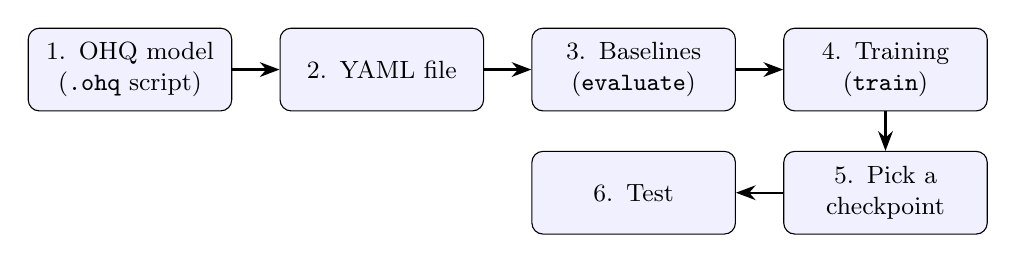
\begin{tikzpicture}[node distance=0.5cm and 0.6cm,
  box/.style={draw, rounded corners, fill=blue!6, align=center, minimum height=1.05cm, text width=2.35cm, font=\small},
  arr/.style={-{Stealth[length=2.5mm]}, thick}]
\node[box] (m) {1. OHQ model\\(\code{.ohq} script)};
\node[box, right=of m] (y) {2. YAML file};
\node[box, right=of y] (b) {3. Baselines\\(\code{evaluate})};
\node[box, right=of b] (t) {4. Training\\(\code{train})};
\node[box, below=of t] (s) {5. Pick a\\checkpoint};
\node[box, left=of s] (x) {6. Test};
\draw[arr] (m) -- (y); \draw[arr] (y) -- (b); \draw[arr] (b) -- (t);
\draw[arr] (t) -- (s); \draw[arr] (s) -- (x);
\end{tikzpicture}
\end{center}
Always evaluate simple fixed controls (step 3) before training. They
tell you how good a policy must be to be worth having. Often a
well-chosen fixed setting is already hard to beat.

%======================================================================
\section{Installation}

\subsection{Requirements}
\begin{itemize}[nosep]
\item OpenHydroQual source tree (this repository), with \code{OHQLib} and
  \code{PythonBindings} built. The bindings must include the stepping API
  (commit \code{c9b9d2b} or later).
\item Python 3.10 or newer, with \code{numpy}, \code{torch},
  \code{gymnasium} and \code{pyyaml} (\code{ohqrl/requirements.txt}).
\item A multi-core CPU. Each training worker runs one OHQ model on one core.
\end{itemize}

\subsection{Build the library and the Python bindings}
With Qt and the OHQ dependencies installed (as for the OHQ GUI), build
\code{OHQLib} first and then the bindings:
\begin{lstlisting}[language=bash]
cd OHQLib && mkdir -p build/Release && cd build/Release
qmake ../../OHQLib.pro CONFIG+=release && make -j8
cd ../../../PythonBindings && mkdir -p build/Release && cd build/Release
qmake ../../PythonBindings.pro CONFIG+=release && make -j8
\end{lstlisting}
\code{PythonBindings.pro} sets the include paths of \code{pybind11} and
Python, and the location of \code{OHQLib}. Adjust them for your system and
build folder names. The build produces \code{openhydroqual\_py*.so} (Linux,
macOS) or \code{.pyd} (Windows).

\subsection{Python environment}
\begin{lstlisting}[language=bash]
python -m venv ~/ohq_env && source ~/ohq_env/bin/activate
pip install -r ohqrl/requirements.txt
\end{lstlisting}

\subsection{Where ohqrl finds OHQ}
Run all commands from the OpenHydroQual folder, so that \code{python -m
ohqrl...} finds the package. By default \code{ohqrl} looks for:
\begin{itemize}[nosep]
\item the bindings under \code{PythonBindings/build/*/}, preferring a
  folder whose name contains \code{Release};
\item the templates in \code{resources/}.
\end{itemize}
Two environment variables override these defaults:
\begin{center}\small
\begin{tabular}{@{}ll@{}}
\toprule
\code{OHQ\_PY\_PATH} & folder that contains \code{openhydroqual\_py*.so}/\code{.pyd}\\
\code{OHQ\_RESOURCES} & folder with the OHQ JSON templates (\code{main\_components.json}, \ldots)\\
\bottomrule
\end{tabular}
\end{center}

\subsection{Check the installation}
\begin{lstlisting}[language=bash]
python -m ohqrl.tests.test_stepping
\end{lstlisting}
The test runs a small reservoir twice. The first time it uses one call to
\code{solve()}. The second time it steps interval by interval and rewrites
the control before each interval. It prints matching storages and
objective values, and \code{OK}.

%======================================================================
\section{Preparing the OHQ model}
\label{sec:model}

\subsection{The script}
The model is an OHQ script (the format written by \emph{File $\to$ Save
as script} in the GUI, or by hand). Two placeholders are replaced before
the script is loaded, so that the model folder can be moved:
\begin{center}\small
\begin{tabular}{@{}ll@{}}
\toprule
\code{\$\{OHQ\_RESOURCES\}} & the OHQ template folder\\
\code{\$\{CONFIG\_DIR\}} & the folder of the YAML file (for forcing files next to it)\\
\bottomrule
\end{tabular}
\end{center}
\begin{lstlisting}
loadtemplate; filename = ${OHQ_RESOURCES}main_components.json
addtemplate; filename = ${OHQ_RESOURCES}Pond_Plugin.json
create block;type=Pond,Storage=0,alpha=250,beta=2,inflow=${CONFIG_DIR}/inflow.txt,name=Pond
\end{lstlisting}
The simulation start and end times in the script are irrelevant: each
episode sets its own. Forcing time series (such as \code{inflow}) should
cover the whole period that episodes are drawn from.

\subsection{Time units}
\code{ohqrl} uses the model's time unit throughout, usually days. All times
in the YAML file (control interval, episode length, windows) are in that
unit. The pond example counts days since 1900-01-01, so 1 hour is
$1/24 = 0.0416667$.

\subsection{Controls}
A control is a property of a block or link that the policy sets. There are
two kinds:
\begin{description}[style=nextline]
\item[\code{value}] An ordinary numeric property, for example the
  \code{opening} of a \code{controlled\_orifice}, or the \code{Q\_max} of a
  \code{Reservoir\_link\_rule}. It is set with \code{set\_value} before
  each interval.
\item[\code{timeseries}] A time-series property, for example the
  \code{flow} of a \code{User\_flow} link or a pump's
  \code{coefficient\_time\_series}. Before each interval it is replaced by
  a constant series holding the chosen value.
\end{description}
The property must be defined in the script (any initial value) and must
actually drive the flow. A property that is only read at initialization
does not respond to changes during the run.

\subsection{Objective functions}
\label{sec:objectives}
Objective functions are created in the script. The \code{type} must be the
template name \code{Objective\_Function}; otherwise the script fails to
load. The \code{method} must be \code{integrate}:
\begin{lstlisting}
create objectivefunction;type=Objective_Function,name=Flood,object=outlet_pipe,expression=(_pos(flow-1000)*_pos(flow-1000)/1000),method=integrate,weight=1
create objectivefunction;type=Objective_Function,name=Young,object=outlet_pipe,expression=(flow*Age:concentration.s),method=integrate,weight=1
\end{lstlisting}
The expression is evaluated on the named block or link at every solver
step, and its time integral is the objective. On a link, \code{.s} and
\code{.e} refer to the quantities of its start and end blocks.

\paragraph{Writing an objective as an integral.} Many goals are naturally
additive. Others can be made so:
\begin{center}\small
\begin{tabular}{@{}p{4.4cm}p{6.2cm}p{3.6cm}@{}}
\toprule
Goal & Expression (integrated) & Comment\\
\midrule
spilled or overflow volume & \code{flow} (on the spill link) & exact\\
pollutant load & \code{flow*C.s} & exact\\
time above a threshold & \code{\_pos(depth-h)/(depth-h+1e-9)} & smooth-ish indicator\\
peak flow / flood exposure & \code{\_pos(flow-Q)*\_pos(flow-Q)/Q} & penalizes large exceedances most\\
exceedance flow at probability $p$ & as above, with $Q$ near the target exceedance flow & surrogate\\
target storage or level & \code{(Storage-S)*(Storage-S)/S} & tracking\\
supply shortfall & \code{\_pos(demand-supply)} & demand as a time series\\
\bottomrule
\end{tabular}
\end{center}
Use squared excesses when large exceedances matter more than many small
ones.

\paragraph{Weights and scales.} Objectives often differ by orders of
magnitude. Give each a \code{scale} in the YAML file, for example its
value per year under a reference control, so that the weighted sum adds
comparable numbers. \code{ohqrl.evaluate --normalize} prints each objective
divided by the baseline's, which helps to choose scales.

%======================================================================
\section{The YAML file}
\label{sec:yaml}

\subsection{Complete example}
\begin{lstlisting}[language=yaml]
model:
  script: pond.ohq                        # relative to this file
  settings:                               # extra OHQ system settings
    initial_time_step: 0.0034722          # 5 min
    max_timestep_increase_factor: 1
time:
  control_interval: 0.0416666667          # 1 h (model time unit: days)
  episode_length: 1095                    # 3 years
  train: [[29219, 43829]]                 # 1980-2019
  validation_starts: [35209, 40104]
  test_starts: [43829, 44925]             # 2020-2022, 2023-2025
controls:
  - {name: valve, object: valve, property: opening, kind: value, min: 0, max: 1, scale: square}
observations:
  - {object: Pond, quantity: Storage, scale: 1000}
  - {object: Pond, quantity: "Age:concentration"}
  - {forcing: inflow.txt, windows: [[-1, 0], [0, 1], [0, 6], [0, 24]],
     scale: 1000, transform: log1p, noise: 0.3}
  - {season: 365.25}
objectives:
  - {name: Flood, weight: 1, scale: 12684}
  - {name: Young, weight: 1, scale: 18982}
snap:
  - {object: Pond, quantity: Storage, below: 0.1}
baseline: {valve: 1.0}
solver_failure_penalty: 10
training:
  total_steps: 3000000
  workers: 8
  warm_start: {controls: {valve: 0.1}}
\end{lstlisting}

\subsection{Reference}
\small
\begin{longtable}{@{}p{3.6cm}p{2.4cm}p{8.6cm}@{}}
\toprule
Key & Default & Meaning\\
\midrule
\endhead
\multicolumn{3}{@{}l}{\textbf{model}}\\
\code{script} & required & OHQ script, relative to the YAML file\\
\code{settings} & \{\} & system settings applied after loading (any OHQ \code{setvalue; object=system} quantity)\\
\midrule
\multicolumn{3}{@{}l}{\textbf{time}} (model time units)\\
\code{control\_interval} & required & $\Delta t$: how often the policy acts\\
\code{episode\_length} & required & $T$: length of one episode\\
\code{train} & required & list of \code{[start, end]} ranges; episodes start uniformly at random in them, on multiples of $\Delta t$, and must fit inside\\
\code{validation\_starts} & [] & start times of fixed windows for choosing among checkpoints (inside the training period)\\
\code{test\_starts} & [] & start times of fixed windows for the final comparison (outside the training period)\\
\midrule
\multicolumn{3}{@{}l}{\textbf{controls} (list; one action per entry)}\\
\code{name} & object.property & label used in \code{baseline}, \code{warm\_start} and \code{--constant}\\
\code{object}, \code{property} & required & block or link name, and the property set\\
\code{kind} & \code{value} & \code{value} or \code{timeseries}\\
\code{min}, \code{max} & required & range of the control\\
\code{scale} & \code{linear} & how the action $a\in[-1,1]$ maps to the range, with $x=(a+1)/2$:
  \code{linear} $u=\min+x(\max-\min)$; \code{square} $u=\min+x^2(\max-\min)$ (finer near \code{min});
  \code{log} $u=\min(\max/\min)^x$ (needs $\min>0$)\\
\midrule
\multicolumn{3}{@{}l}{\textbf{observations} (list; each entry is one of three kinds)}\\
\code{object}, \code{quantity} & -- & a state or other quantity, e.g. \code{Storage}, \code{depth}, \code{"Age:concentration"}\\
\code{forcing} & -- & a two-column file (time, value; comma separated); one input per window\\
\code{windows} & [[0, 1]] & for \code{forcing}: list of \code{[a, b]} in control intervals; the input is the mean over $[t+a\Delta t,\,t+b\Delta t]$; windows with $b>0$ are forecasts\\
\code{noise} & 0 & for \code{forcing}: log-normal forecast error (standard deviation of the log) applied to forecast windows\\
\code{season} & -- & period (e.g.\ 365.25); adds $\sin$ and $\cos$ of the phase\\
\code{scale} & 1 & divide by this (aim for values of order one)\\
\code{transform} & \code{none} & \code{none} or \code{log1p} (after scaling; for skewed inputs such as flows)\\
\midrule
\multicolumn{3}{@{}l}{\textbf{objectives} (list)}\\
\code{name} & required & an objective function in the script (method \code{integrate})\\
\code{weight} & 1 & multiplies OHQ's own weight\\
\code{scale} & 1 & divides the objective\\
\midrule
\multicolumn{3}{@{}l}{\textbf{optional}}\\
\code{initial\_state} & [] & \code{\{object, quantity, uniform: [lo, hi]\}}: random initial state for training episodes\\
\code{snap} & [] & \code{\{object, quantity, below\}}: before each interval, a value with $|x|<$ \code{below} is set to 0\\
\code{baseline} & \{\} & reference fixed controls \code{\{name: value\}} (first row of every evaluation)\\
\code{solver\_failure\_penalty} & 10 & reward when the OHQ solve fails (the episode then ends)\\
\midrule
\multicolumn{3}{@{}l}{\textbf{training} (all optional)}\\
\code{total\_steps} & 1\,000\,000 & control intervals simulated in total (all workers)\\
\code{workers} & 8 & parallel OHQ models (CPU cores)\\
\code{rollout\_steps} & 256 & intervals per worker between updates\\
\code{gamma} & 0.99 & discount per interval; the policy looks about $1/(1-\gamma)$ intervals ahead\\
\code{lam} & 0.95 & GAE parameter\\
\code{lr}, \code{epochs}, \code{minibatch} & 3e-4, 10, 256 & optimizer settings\\
\code{clip}, \code{vf\_coef}, \code{ent\_coef} & 0.2, 0.5, 0 & PPO settings\\
\code{normalize\_rewards} & true & scale rewards by the running standard deviation of the return\\
\code{reward\_clip} & 0 & clip normalized rewards ($0$: off)\\
\code{save\_every} & 25 & checkpoint every N updates\\
\code{seed} & 0 & random seed\\
\code{warm\_start} & none & start from a simple rule (Section~\ref{sec:warm})\\
\bottomrule
\end{longtable}
\normalsize

%======================================================================
\section{Running}

All commands are run from the OpenHydroQual folder.

\subsection{Step 1: baselines}
\begin{lstlisting}[language=bash]
python -m ohqrl.evaluate model.yaml --windows validation \
    --constant "valve=0.05" "valve=0.1" "valve=0.2" --normalize --log baselines.json
\end{lstlisting}
Every evaluation runs the \code{baseline} controls first, then the
policies you list. The \code{--constant} option takes comma-separated
assignments for several controls, e.g.\ \code{"gate=0.3,pump=50"}. Each
policy is run on every window, without randomness. The script prints:
\begin{description}[nosep]
\item[\code{J}] the weighted objective, $\sum_i w_i\omega_i I_i/s_i$,
  averaged over the windows. Lower is better.
\item[objective values] the integral of each objective function over the
  window, i.e.\ OHQ's objective value.
\item[\code{normalized}] each objective divided by the baseline's (with
  \code{--normalize}).
\end{description}
Use the validation windows to choose among fixed settings. The test
windows are kept for the end.

\subsection{Step 2: training}
\begin{lstlisting}[language=bash]
python -m ohqrl.train model.yaml --out runs/model1
python -m ohqrl.train model.yaml --out runs/model2 --total-steps 500000 --workers 16
\end{lstlisting}
Command-line options override the \code{training} section. The run folder
receives \code{config.yaml}, \code{train\_log.txt}, the checkpoints
\code{checkpoint\_uNNNN.pt} and \code{final.pt}. Each line of the log is one
update:
\begin{center}\small
\begin{tabular}{@{}lp{10.5cm}@{}}
\toprule
\code{intervals} & control intervals simulated so far\\
\code{episodes} & complete episodes so far\\
\code{mean episode return} & average total reward of the last 20 episodes (higher is better). It is measured \emph{with exploration noise} and on random windows, so it is noisy and does not by itself show that the policy improved\\
\code{exploration std} & spread of the random exploration around the policy's action (in action units, $[-1,1]$)\\
\code{intervals/s} & simulation speed\\
\bottomrule
\end{tabular}
\end{center}
\textbf{Run time.} Roughly
$\text{total\_steps} / (\text{workers}\times\text{intervals per second per worker})$.
The pond example runs at about 30--40 intervals per second per worker.

\subsection{Step 3: choose a checkpoint}
\begin{lstlisting}[language=bash]
python -m ohqrl.evaluate model.yaml --windows validation \
    --ppo "runs/model1/checkpoint_u*.pt" --select runs/model1/best.pt --log runs/model1/selection.json
\end{lstlisting}
Every checkpoint is run without exploration noise on the validation
windows. The one with the lowest \code{J} is copied to \code{best.pt}.
Choose this way rather than taking the last checkpoint. RL training is
noisy, and later is not always better. Checkpoint \code{u0000} is the
starting policy (the warm-start rule), so the selected policy is never
worse than that rule on the validation windows.

\subsection{Step 4: test}
\begin{lstlisting}[language=bash]
python -m ohqrl.evaluate model.yaml --windows test \
    --constant "valve=0.05" --ppo runs/model1/best.pt --normalize --log runs/model1/test.json
\end{lstlisting}
Compare the trained policy with the best fixed setting on windows that
played no role in training or selection.

\subsection{Warm start}
\label{sec:warm}
Starting PPO from a reasonable rule saves most of the training time. The
actor network is first fitted to the rule's actions (behavior cloning),
then improved. Two forms are available:
\begin{lstlisting}[language=yaml]
training:
  warm_start: {controls: {valve: 0.1}}                     # fixed controls
  # or: warm_start: {rule: "mymodule:my_rule", kwargs: {threshold: 0.5}}
  # optional: steps (per worker, 2000), epochs (30), log_std (-1.6)
\end{lstlisting}
A rule is a Python function \code{my\_rule(env, **kwargs)} that returns the
action vector, with one entry in $[-1,1]$ per control. Inside the rule,
\code{env.sys} is the live OHQ model (e.g.\ \code{env.sys.get\_value("Pond",
"Storage")}) and \code{env.t} the current time.
\code{env.action\_from\_control(c, u)} converts a control value to an
action. \code{log\_std} sets the exploration spread after cloning, as the
natural logarithm of the standard deviation in action units ($-1.6$ means
$0.2$).

%======================================================================
\section{Worked example: stormwater pond}

\code{ohqrl/examples/pond} contains a stormwater pond with a controllable
outlet valve:
\begin{itemize}[nosep]
\item \textbf{Inflow:} hourly runoff from a 2-ha impervious catchment, using
  the 1979--2025 rain record of Beltsville, MD (NOAA station
  USC00180700).
\item \textbf{Layout:} the valve and an overflow weir discharge into a catch
  basin, which drains through a pipe to the outlet.
\item \textbf{Water age:} a Laplace age tracer measures how ``young'' the
  outflow is.
\end{itemize}
There are two objectives:
\begin{itemize}[nosep]
\item \code{Flood}: the integral of the squared outlet-flow excess above
  1000~m$^3$/d;
\item \code{Young}: the integral of outflow times tracer concentration, i.e.\
  the young-water load.
\end{itemize}
Both are scaled by their values per year with the valve fully open, so
the passive pond scores 1 per objective per year.

\begin{lstlisting}[language=bash]
python ohqrl/examples/pond/make_inputs.py
python -m ohqrl.evaluate ohqrl/examples/pond/pond.yaml --windows test \
    --constant "valve=0.05" "valve=0.1" "valve=0.2" --normalize
\end{lstlisting}
\begin{center}\small
\begin{tabular}{@{}lrrr@{}}
\toprule
Fixed opening & $J$ (test, 2 windows of 3 yr) & Flood / passive & Young / passive\\
\midrule
100\% (passive) & 8.24 & 1.000 & 1.000\\
20\% & 3.33 & 0.039 & 0.926\\
10\% & 2.80 & 0.005 & 0.820\\
5\% & 2.35 & 0.029 & 0.655\\
\bottomrule
\end{tabular}
\end{center}
A small fixed opening already removes almost all of the flood objective
and a third of the young-water load. A trained policy has to beat 2.35 to
be worth having. It could do so, for example, by keeping the valve nearly
closed in dry weather (aging the water) and opening it before forecast
storms. Training follows with \code{python -m ohqrl.train
ohqrl/examples/pond/pond.yaml --out runs/pond}, then Steps~3--4.

%======================================================================
\section{Using the environment from Python}

\code{OHQControlEnv} is a standard Gymnasium environment, so it can be used
with any RL library or with your own optimization loop:
\begin{lstlisting}[language=python]
from ohqrl.env import OHQControlEnv, constant_policy
env = OHQControlEnv("ohqrl/examples/pond/pond.yaml")
obs, info = env.reset(seed=1, options={"start": 43829, "initial_state": {}})
done = False
while not done:
    action = constant_policy(env, {"valve": 0.05})      # or your policy(obs)
    obs, reward, terminated, truncated, info = env.step(action)
    done = terminated or truncated
print(env.objective_totals())                           # OHQ objective values for the window
env.close()
\end{lstlisting}
\code{reset} options:
\begin{itemize}[nosep]
\item \code{start}: a fixed start time; otherwise a random training start.
\item \code{initial\_state}: \code{\{(object, quantity): value\}}, which
  replaces the random initial state. An empty dictionary keeps the
  script's values.
\end{itemize}
\code{info} contains the time, the control values applied, and the
objective increments of the interval.

\subsection{The OHQ stepping API}
The environment rests on these methods of \code{openhydroqual\_py.System},
which are also usable directly:
\begin{center}\small
\begin{tabular}{@{}p{6.2cm}p{8.6cm}@{}}
\toprule
\code{begin\_stepping(apply\_parameters)} & initialize the solver as \code{solve()} does, without running\\
\code{advance\_to(t)} & continue the run to time $t$ without re-initializing; \code{False} if the solve failed\\
\code{end\_stepping(uniformize\_output)} & finalize the outputs\\
\code{current\_time()}, \code{start\_time()}, \code{end\_time()} & simulation times\\
\code{get\_value(obj, q)}, \code{get\_values([(obj, q), ...])} & current value(s) of quantities\\
\code{set\_value(obj, q, v)} & set a quantity now (present and past values)\\
\code{set\_timeseries(obj, prop, t, v)} & replace a time-series property\\
\code{set\_block\_property}, \code{set\_link\_property} & set a property by its text value\\
\code{objective\_names()}, \code{objective\_method(n)}, \code{objective\_weight(n)} & objective functions in the model\\
\code{objective\_integral(n)} & integral of objective $n$ from the start of the run to now\\
\code{objective\_value(n)} & the objective as OHQ evaluates it (its method)\\
\bottomrule
\end{tabular}
\end{center}

%======================================================================
\section{Practical advice}

\subsection{Speed}
\begin{itemize}
\item The OHQ solve is almost all of the cost. Use the largest solver step
  (\code{initial\_time\_step}) that is accurate, and
  \code{max\_timestep\_increase\_factor: 1} if the step should not grow.
\item Near-empty storages left at round-off levels (around $10^{-9}$) can
  slow the solver by orders of magnitude. List them under \code{snap}. In
  the pond example, a 30-day test that took 94~s (and then failed) without
  snapping ran in 3~s with it.
\item A long control interval means fewer decisions per episode and faster
  training, at the cost of a less responsive policy.
\item Set \code{make\_timeseries\_uniform: no} (already in the example
  script) when forcing files are long: resampling a multi-decade record at
  every episode start is slow.
\end{itemize}

\subsection{Long runs}
An episode is one long OHQ run. \code{ohqrl} raises OHQ's whole-run limits
on matrix inversions (\code{maximum\_number\_of\_matrix\_inverstions}, so
spelled in OHQ) and wall-clock time (\code{maximum\_time\_allowed}). Without
this, multi-year episodes fail partway. Both can be overridden under
\code{model: settings}.

\subsection{Getting a policy that is really better}
These lessons come from the reservoir, pond and environmental-flow studies
in the OpenHydroQual-RL project:
\begin{enumerate}
\item \textbf{Tune the simple rules first.} A grid of fixed settings, or a
  simple threshold rule, is often hard to beat. Report the trained policy
  against the \emph{best} of them.
\item \textbf{Train on what you evaluate.} \code{ohqrl} guarantees this:
  the reward sums to the objective. If you add terms of your own, keep them
  consistent with how you will judge the result. Otherwise RL optimizes the
  difference.
\item \textbf{Judge without noise.} The training curve includes exploration
  noise. Always select and test with \code{ohqrl.evaluate}, which runs the
  policy deterministically.
\item \textbf{Exploration noise can bias the result.} If small, random
  changes of the control are themselves penalized, the noisy training
  policy is worse than the policy it is learning, and training drifts.
  Examples are thresholds that a slightly lower release misses, and limits
  on day-to-day changes. Use smooth objectives, a smaller \code{log\_std}
  after the warm start, or a longer control interval.
\item \textbf{Look ahead far enough.} The policy weighs rewards about
  $1/(1-\gamma)$ intervals ahead. Make that horizon cover the effect of a
  decision, e.g.\ a storm event for a pond, or a season for a reservoir.
  \code{gamma} close to 1 trains more slowly.
\item \textbf{Keep test windows out of every decision}, including the
  choice of scales, rule settings and checkpoints.
\end{enumerate}

\subsection{Troubleshooting}
\begin{center}\small
\begin{longtable}{@{}p{5.3cm}p{9.2cm}@{}}
\toprule
Symptom & Cause and remedy\\
\midrule
\endhead
\code{openhydroqual\_py not found} & bindings not built, or in an unexpected folder: set \code{OHQ\_PY\_PATH}\\
\code{OHQ could not build the model} & script error. Load it in the OHQ GUI or run it with the terminal version for messages. Objective functions need \code{type=Objective\_Function}\\
\code{... uses method 'maximum'} & only \code{integrate} objectives are accepted: rewrite as an integral (Section~\ref{sec:objectives})\\
\code{KeyError: not found: X:Y} & block/link \code{X} has no quantity \code{Y}; check names and capitalization (\code{Storage}, \code{depth}, \code{"Age:concentration"})\\
episodes end early with \code{solver\_failed} & the OHQ solve failed: smaller \code{initial\_time\_step}, \code{snap} near-zero states, check the model alone over the same window\\
very slow intervals & round-off states (use \code{snap}), very small solver steps, or many workers on few cores\\
control has no effect & the property is not used by the flow expression after initialization, or the wrong \code{kind}\\
\code{no training range is longer than the episode} & \code{train} ranges shorter than \code{episode\_length}\\
\bottomrule
\end{longtable}
\end{center}

\subsection{Limitations}
\begin{itemize}[nosep]
\item Objectives must be additive (time integrals).
\item The policy sees only what is listed under \code{observations}. Hidden
  states that matter should be included.
\item The bundled trainer is PPO with small fully connected networks.
  Other algorithms can use \code{OHQControlEnv} directly.
\item Each worker rebuilds the model from the script at every episode
  start. This is cheap compared with an episode, but not free for very
  large models.
\end{itemize}

\end{document}
